\documentclass[11pt]{article}
\usepackage{fullpage}
\usepackage{comment}
\usepackage{amssymb}
\usepackage{hyperref}
\newcommand{\cd}{\cdot}
\usepackage{graphicx}
\setlength{\parindent}{0pt}
\setlength{\parskip}{0.3cm}
\newcommand{\nats}{\mathbb{N}}
\newcommand{\ints}{\mathbb{Z}}
\newcommand{\nnot}{\mathrm{NOT}}
\includecomment{soln}
\begin{document}
\begin{center}
{\bf \Large \bf CSC240 Winter 2024 Quiz 9}\\
due April 5, 2024
\end{center}
Consider the DFA $M=(\{ q_0,q_1, q_2\}, \{0,1,2\}, \delta, q_0, \{q_0\})$, where\\
$\delta(q_i , 0 ) = q_i$ for all $i \in \{0,1,2\}$,\\
$\delta(q_i , 1 ) = q_{i+1}$ for all $i \in \{0,1\}$,\\
$\delta(q_2 , 1 ) = q_0$,\\
$\delta(q_0 , 2 ) = q_2$, and\\
$\delta(q_i , 2 ) = q_{i-1}$ for all $i \in \{1,2\}$.

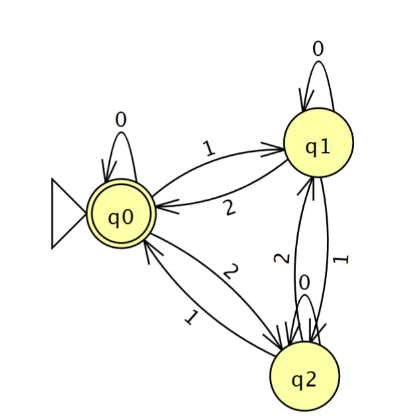
\includegraphics[scale=0.5]{img/2024-04-05-01-14-32.png}

\begin{enumerate}
\item
Describe the language $ L(M)= \{ x \in \{0,1,2\}^* \mid \ldots\ \}$ by replacing
the $\ldots$ with at most 15 words.
Do not mention $\delta$.

Here $\ldots$ is equivalent to ``the sum of the letters in $x$ is divisible by 3.''


\item
Construct a regular expression $r$ such that $L(r) = L(M)$.

Construct 
\begin{verbatim}
r=(
    0
    + (2(0)*1)
    + (1(0)*2)
    + ((1 + 2(0)*2) (0 + 1(0)*2)* (2 + 1(0)*1) (0 + 2(0)*1)*)
)*
\end{verbatim}

Or in 1 line: $r=(0 + (20^*1) + (10^*2) + ((1 + 20^*2) (0 + 10^*2)^* (2 + 10^*1) (0 + 20^*1)^*))^*$

Then we can claim that $L(r)=L(M)$.


\end{enumerate}
\end{document}
